% The document class supplies options to control rendering of some standard
% features in the result.  The goal is for uniform style, so some attention
% to detail is *vital* with all fields.  Each field (i.e., text inside the
% curly braces below, so the MEng text inside {MEng} for instance) should
% take into account the following:
%
% - author name       should be formatted as "FirstName LastName"
%   (not "Initial LastName" for example),
% - supervisor name   should be formatted as "Title FirstName LastName"
%   (where Title is "Dr." or "Prof." for example),
% - degree programme  should be "BSc", "MEng", "MSci", "MSc" or "PhD",
% - dissertation title should be correctly capitalised (plus you can have
%   an optional sub-title if appropriate, or leave this field blank),
% - dissertation type should be formatted as one of the following:
%   * for the MEng degree programme either "enterprise" or "research" to
%     reflect the stream,
%   * for the MSc  degree programme "$X/Y/Z$" for a project deemed to be
%     X%, Y% and Z% of type I, II and III.
% - year              should be formatted as a 4-digit year of submission
%   (so 2014 rather than the accademic year, say 2013/14 say).

\documentclass[ % the name of the author
                    author={Alexander Hill},
                % the name of the supervisor
                supervisor={Dr. Benjamin Sach},
                % the degree programme
                    degree={MEng},
                % the dissertation    title (which cannot be blank)
                     title={MARMOSET: Multi Agent Real-time Multi-core Online
                     Simulation for Efficient Transportation},
                % the dissertation subtitle (which can    be blank)
                  subtitle={},
                % the dissertation     type
                      type={research},
                % the year of submission
                      year={2016} ]{dissertation}

\setlength{\parskip}{1em}
\usepackage{tikz}
\usetikzlibrary{matrix,arrows,positioning}
\usepackage{wrapfig}
\usepackage{caption}
\usepackage{subcaption}

\graphicspath{ {images/} }

\begin{document}

% =============================================================================

% This macro creates the standard UoB title page by using information drawn
% from the document class (meaning it is vital you select the correct degree
% title and so on).

\maketitle

% After the title page (which is a special case in that it is not numbered)
% comes the front matter or preliminaries; this macro signals the start of
% such content, meaning the pages are numbered with Roman numerals.

\frontmatter

% This macro creates the standard UoB declaration; on the printed hard-copy,
% this must be physically signed by the author in the space indicated.

\makedecl

% LaTeX automatically generates a table of contents, plus associated lists
% of figures, tables and algorithms.  The former is a compulsory part of the
% dissertation, but if you do not require the latter they can be suppressed
% by simply commenting out the associated macro.

\tableofcontents
\listoffigures
\listoftables
\listofalgorithms
\lstlistoflistings

% The following sections are part of the front matter, but are not generated
% automatically by LaTeX; the use of \chapter* means they are not numbered.

% -----------------------------------------------------------------------------

\chapter*{Executive Summary}

{\bf A compulsory section, of at most $1$ page}
\vspace{1cm}

%\noindent
%This section should pr\'{e}cis the project context, aims and objectives,
%and main contributions (e.g., deliverables) and achievements; the same
%section may be called an abstract elsewhere.  The goal is to ensure the
%reader is clear about what the topic is, what you have done within this
%topic, {\em and} what your view of the outcome is.

%The former aspects should be guided by your specification: essentially
%this section is a (very) short version of what is typically the first
%chapter.  Note that for research-type projects, this {\bf must} include
%a clear research hypothesis.  This will obviously differ significantly
%for each project, but an example might be as follows:

%\begin{quote}
%My research hypothesis is that a suitable genetic algorithm will yield
%more accurate results (when applied to the standard ACME data set) than
%the algorithm proposed by Jones and Smith, while also executing in less
%time.
%\end{quote}

%\noindent
%The latter aspects should (ideally) be presented as a concise, factual
%bullet point list.  Again the points will differ for each project, but
%an might be as follows:

%\begin{quote}
%\noindent
%\begin{itemize}
%\item I spent $120$ hours collecting material on and learning about the
      %Java garbage-collection sub-system.
%\item I wrote a total of $5000$ lines of source code, comprising a Linux
      %device driver for a robot (in C) and a GUI (in Java) that is
      %used to control it.
%\item I designed a new algorithm for computing the non-linear mapping
      %from A-space to B-space using a genetic algorithm, see page $17$.
%\item I implemented a version of the algorithm proposed by Jones and
      %Smith in [6], see page $12$, corrected a mistake in it, and
      %compared the results with several alternatives.
%\end{itemize}
%\end{quote}

% -----------------------------------------------------------------------------

\chapter*{Supporting Technologies}

\noindent
This project has two parts - a back end engine written in Java, and a front end
visualisation part running in the browser using JavaScript.

\subsection*{Back End}
\begin{quote}
\noindent
\begin{itemize}
    \item OpenStreetMaps (OSM)~\cite{osm} is used for the raw mapping data. Specific sections of
        the maps can be downloaded from Geofabrik.
    \item The Open Source routing engine GraphHopper~\cite{graphhopper} was
        used for performing basic routing requests and handling storage and
        processing of the OpenStreetMaps data.
    \item NanoHttpd~\cite{nanohttpd} was used for a static file server to
        provide HTML, CSS and images to the front end.
    \item Java WebSocket~\cite{javawebsocket} was used for communication
        between the front and back end.
\end{itemize}
\end{quote}

\subsection*{Front End}
\begin{quote}
\noindent
\begin{itemize}
    \item The map interface on the front end uses the JavaScript library
        Leaflet.js~\cite{leaflet} for the map and marker APIs.
    \item Mapbox is used for the image tiles to display the underlying map.
\end{itemize}
\end{quote}


% -----------------------------------------------------------------------------

\chapter*{Notation and Acronyms}

%{\bf An optional section, of roughly $1$ or $2$ pages}
%\vspace{1cm}

%\noindent
%Any well written document will introduce notation and acronyms before
%their use, {\em even if} they are standard in some way: this ensures
%any reader can understand the resulting self-contained content.

%Said introduction can exist within the dissertation itself, wherever
%that is appropriate.  For an acronym, this is typically achieved at
%the first point of use via ``Advanced Encryption Standard (AES)'' or
%similar, noting the capitalisation of relevant letters.  However, it
%can be useful to include an additional, dedicated list at the start
%of the dissertation; the advantage of doing so is that you cannot
%mistakenly use an acronym before defining it.  A limited example is
%as follows:

\begin{quote}
\noindent
\begin{tabular}{lcl}
OSM                 &:     & OpenStreetMap \\
\end{tabular}
\end{quote}

% -----------------------------------------------------------------------------

\chapter*{Acknowledgements}

{\bf An optional section, of at most $1$ page}
\vspace{1cm}

% Thank Ben, Peter Karich, Pie Mapping

%\noindent
%It is common practice (although totally optional) to acknowledge any
%third-party advice, contribution or influence you have found useful
%during your work.  Examples include support from friends or family,
%the input of your Supervisor and/or Advisor, external organisations
%or persons who  have supplied resources of some kind (e.g., funding,
%advice or time), and so on.

% =============================================================================

% After the front matter comes a number of chapters; under each chapter,
% sections, subsections and even subsubsections are permissible.  The
% pages in this part are numbered with Arabic numerals.  Note that:
%
% - A reference point can be marked using \label{XXX}, and then later
%   referred to via \ref{XXX}; for example Chapter\ref{chap:context}.
% - The chapters are presented here in one file; this can become hard
%   to manage.  An alternative is to save the content in seprate files
%   the use \input{XXX} to import it, which acts like the #include
%   directive in C.

\mainmatter

% -----------------------------------------------------------------------------

\chapter{Contextual Background}
\label{chap:context}

\vspace{1cm}

\noindent

\section{Routing in the 21st Century} % retitled introduction?

When MapQuest first launched in 1996, most drivers found their way to new
locations using physical paper maps as well as knowledge gained through
experience. MapQuest was the first online service to change that - instead of
figuring out a route yourself, you could enter your location and destination and
have a route provided to you. Unfortunately, using these routes meant printing
out or writing down the instructions yourself - the route was fixed from when it
was calculated.

In 2005, the first online version of Google Maps was released. Unlike its
predecessors, Google Maps used real-time traffic analysis to improve the routes
it offered to its users. However, with the exception of high-end vehicles with
GPS navigation, these were still usually printed for use.

It took the release of the iPhone in 2007 to take full
advantage of the new information available - suddenly, people were able to plan
routes and modify them whilst travelling, whilst Google could use this
information to improve their data on congestion.

\section{Self-Driving Vehicles}

This technology has now been integrated into almost every modern vehicle
available to purchase today. GPS based navigation, with traffic information and
turn by turn routing instructions are standard features in many car models.
Furthermore, we are seeing some further intelligence being added to cars, from
two perspectives.

The first is modifying existing cars - adding features such as
cruise control, automatic braking systems, reading of road signs, lane following
on highways, and so on until eventually the car will need minimal or no human
intervention. This approach is being taken by Tesla, who have released multiple
software updates to their car software that enables further automation by the
car itself. The second approach is from companies like Google, who have been
building a self-driving vehicle `from scratch', creating a vehicle that has no
steering wheel and requires no human intervention to drive from one location to
another.

\section{Congestion}

With the advent of Google Maps and the proliferation of mobile
devices, many drivers are now provided with directions that can incorporate
large amounts of additional information - including current traffic conditions
and road closures. This is particularly important in cities, where the levels of
congestion during `rush hour' can have a drastic impact on travel time.

Looking forwards, we can see two trends that suggest that congestion will become
more of an issue in future. Firstly, more and more people are living in cities -
even with good public transportation, this will increase the number of vehicles
on the road even if it lowers the proportion of households that own cars.
Secondly, on-demand transport solutions (such as those provided by Uber) are
leading to more vehicles on the road, especially at peak times. One of Uber's
key insights is using market techniques to better match supply and demand than
existing taxi and minicab services. If there is an increase in riders requesting
vehicles in a certain area, Uber activates \"surge pricing", increasing the cost
of the ride by a fixed multiple - for example, 1.5x. This information is sent to
their network of drivers, who will move to the location in search of higher
paying riders. The net result of this is that high-demand in certain areas will
create further congestion, even though on demand transportation is usually more
efficient than personal car ownership.

At the same time, we are beginning to witness the rise of self-driving cars,
capable of planning and executing routes themselves with no need for human
intervention. This raises many questions about the role of personal
transportation and the effect this will have on congestion. Will driving become
as dated as horseriding is today - or will people's enjoyment of it mean that
there'll always be human driven vehicles on the road? More importantly, will
self driving cars improve or harm congestion - and how will they decide what
routes they should take?
% could expand upon this with further extensions of long term self-driving
% future, as well as more specific issues that SDVs raise.

Answers to these questions are important to many people, including individual
drivers, companies owning large fleets of vehicles, and city planners. Although
it is not possible to provide definitive answers, simulation provides a
technique for evaluating how future transportation will look and the impact it
may have.

\section{Simulation}

One way of finding answers to these questions is simulation - modelling and
making assumptions about future behaviours and analysing the results. Vehicles
simulation can be used in a number of ways:

\begin{itemize}
    \item Simulating current vehicle behaviour and traffic conditions to
        identify improvements to the road network.
    \item Modifying the road and transport networks (e.g busses, taxis) in the
        simulation to identify the impact changes would have.
    \item Designing and running novel algorithms for simulating self-driving
        vehicles, modelling their behaviour in response to both human drivers
        and other self-driving vehicles.
\end{itemize}

\subsection{Types of Simulation}

\textbf{V2V vs V2I etc}

There are two main tools in use today for running vehicle simulations. The first
is MATSim~\cite{matsim}, and the second is SUMO~\cite{sumo}.

\subsection{MATSim}

\subsection{SUMO}

Existing tools are cumbersome, slow, non-interactive and designed to be used
for any type of multi-agent problem - from routing air traffic to planning for
evacuation in crisis situations. This project aims to create a system designed
exclusively for one goal - road based simulations for vehicles and traffic.
By focussing on a specific use case, a tool can be easier to use, faster to
setup and provide specialised functionalities for our use case.

Additionally, existing tools tend to focus on simulation then visualisation,
without combining the two. Simultaneous simulation and visualisation allows a
much tighter loop of testing and iterating on algorithm design and analysis.



\begin{quote}
\noindent
The high-level objective of this project is to build an easier, faster way of
simulating the behaviour of vehicles, primarily in cities. The concrete aims
are:

\begin{enumerate}
    \item Research existing algorithms and simulation tools to identify the
            strengths and weaknesses of current approaches.
    \item Design a simulation architecture that allows for fast experimentation,
        easy integration with real world information and full implementation
        flexibility.
    \item Build and optimise the simulation engine on top of existing open
        source tools.
    \item Demonstrate the power and flexibility of the engine by experimentally
        creating a novel multi-vehicle routing algorithm.
\end{enumerate}

\end{quote}

%This chapter should describe the project context, and motivate each of
%the proposed aims and objectives.  Ideally, it is written at a fairly
%high-level, and easily understood by a reader who is technically
%competent but not an expert in the topic itself.

%In short, the goal is to answer three questions for the reader.  First,
%what is the project topic, or problem being investigated?  Second, why
%is the topic important, or rather why should the reader care about it?
%For example, why there is a need for this project (e.g., lack of similar
%software or deficiency in existing software), who will benefit from the
%project and in what way (e.g., end-users, or software developers) what
%work does the project build on and why is the selected approach either
%important and/or interesting (e.g., fills a gap in literature, applies
%results from another field to a new problem).  Finally, what are the
%central challenges involved and why are they significant?

%The chapter should conclude with a concise bullet point list that
%summarises the aims and objectives.  For example:

%\begin{quote}
%\noindent
%The high-level objective of this project is to reduce the performance
%gap between hardware and software implementations of modular arithmetic.
%More specifically, the concrete aims are:

%\begin{enumerate}
%\item Research and survey literature on public-key cryptography and
      %identify the state of the art in exponentiation algorithms.
%\item Improve the state of the art algorithm so that it can be used
      %in an effective and flexible way on constrained devices.
%\item Implement a framework for describing exponentiation algorithms
      %and populate it with suitable examples from the literature on
      %an ARM7 platform.
%\item Use the framework to perform a study of algorithm performance
      %in terms of time and space, and show the proposed improvements
      %are worthwhile.
%\end{enumerate}
%\end{quote}

% -----------------------------------------------------------------------------

\chapter{Technical Background}
\label{chap:technical}

%%%%%% ======= 10 PAGES =======

\section{Algorithmic Background}

\subsection{Dijkstra's Algorithm}

Dijkstra's Algorithm~\cite{dijkstra}, originally designed in 1956, forms the
foundation of most modern routing algorithms.

\begin{algorithm}[h]
\SetKwProg{Fn}{Function}{}{}
\DontPrintSemicolon
\SetAlgoLined

    \Fn{\textsc{Dijkstra}(G,s,d)}{
        $Q \leftarrow \textrm{new Priority Queue}$ \;
        $dist[s] \leftarrow 0$ \;
        \For{vertex $v \neq s \in G$}{
            $dist[v] = \infty$ \;
            $prev[v] = undefined$ \;
            $Q.\textrm{add}(v, dist[v])$ \tcp*[h]{Adds $v$ to priority queue with weight $dist[v]$} \;
        }
        \While{$Q \neq \emptyset$}{
            $u \leftarrow Q.\textrm{extract\_min}()$ \;
            \If{$u = d$}{
                $\textbf{Return BuildPath}(u)$
            }
            \For{neighbour $v$ of $u$}{
                $d \leftarrow dist[u] + \textbf{distance}(u,v)$ \;
                \If{$d < dist[v]$}{
                    $dist[v] \leftarrow d$ \;
                    $prev[v] \leftarrow u$ \;
                    $Q.\textrm{decrease\_priority}(v, d)$ \;
                }
            }
        }
    }

\caption{Dijkstra's Algorithm}\label{dij-alg}
\end{algorithm}

The algorithm operates on a graph consisting of nodes connected to each other by
edges. Each edge has a weight - this could be the length of the road in a real
world map. Given two nodes $S$ and $D$, the goal is to return a list of edges that
represents the shortest path between the nodes.

At its core, the algorithm picks the edge with the next shortest distance
from the source node and updates the distance value for that node. It repeats
this process until it finds the source node connected to an edge, then works
backwards to construct the shortest path between the two nodes.

Algorithm \ref{dij-alg} shows how it works in pseudocode. The implementation for
the \textbf{BuildPath} function simply iterates through each nodes parent and
adds it to the output list. We also define the \textbf{distance} function that
simply returns the weight of the edge between vertices $u$ and $v$.

\subsubsection{Bidirectional Dijkstra's Algorithm}

By default, the algorithm searches outwards from only the source. We can improve
the performance of Dijkstra's algorithm by searching backwards from the
destination and forward from the source simultaneously.

\subsubsection{A* Algorithm}

By itself, Dijkstra's algorithm will search all edges based on their cost from
the start node. However, when routing on a real world map this leads to a lot of
wasted work searching in the opposite direction from the destination.

In Dijkstra's algorithm, the distance from the source node is used as the key in
the priority queue (line X). The A* algorithm instead seeks to minimize the
function $f(v) = dist[v] + h(v)$, where $h(v)$ is a heuristic that estimates the
cost to destination.

A bidirectional version of the A* algorithm can also be used for further
improvements to performance.

\begin{figure}[h]
\centering
\begin{subfigure}[b]{0.4\textwidth}
    \centering
    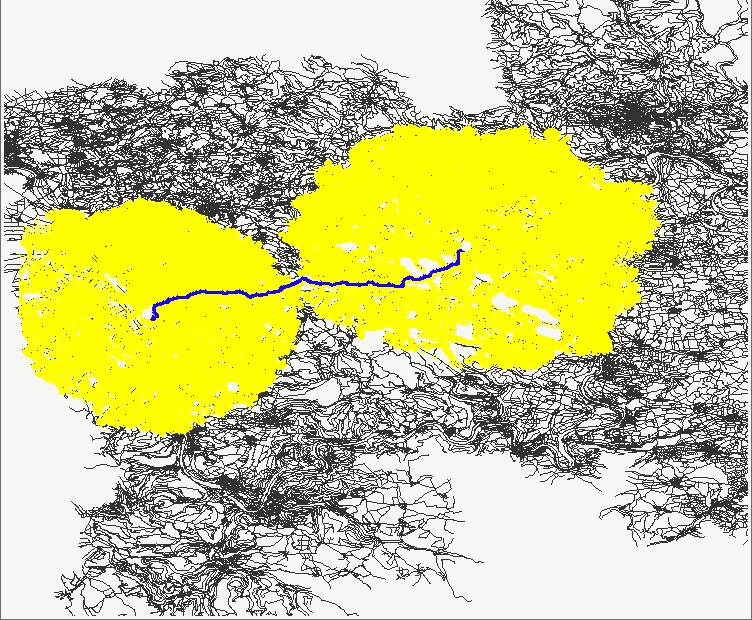
\includegraphics[height=15em]{bidijkstra-city}
    \caption{Dijkstra's Algorithm}\label{fig:bidijkstra}
\end{subfigure}
\hspace{2em}
\begin{subfigure}[b]{0.4\textwidth}
    \centering
    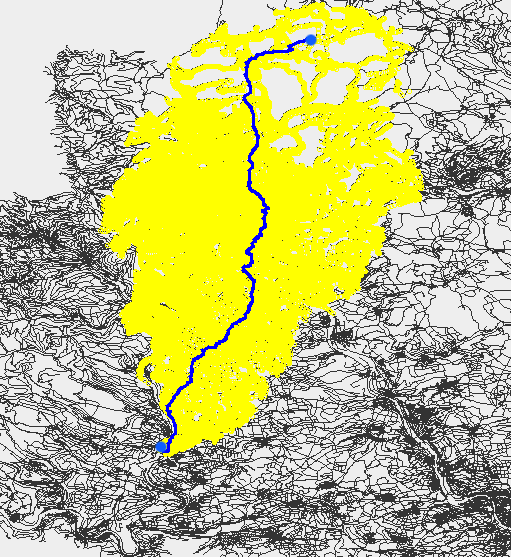
\includegraphics[height=15em]{astar-city}
    \caption{A* Algorithm}\label{fig:astar}
\end{subfigure}
\caption{Paths searched by each algorithm}
\end{figure}

\subsubsection{Contraction Heirarchies}

If the weights on each edge of the graph are known in advance, we can process
the graph to pre-compute the shortest path between certain key nodes in the
graph. One such algorithm for this is the Contraction Heirarchies algorithm,
which works by building shortcuts on top of each other in a heirarchy. It then
uses a modified version of bidirectional Dijkstra's algorithm that only uses
shortcuts higher than the current one to route between two points.

Although they double memory usage, in practice Contraction Heirarchies have a
huge impact on query times. For routing from Moscow to Madrid, any dijkstra based algorithm
takes at least 10 seconds, compared to less than 0.05s for a processed graph.
\textbf{Cite: https://graphhopper.com/public/slides/2014-locationtech.pdf}

\subsection{Nagel-Schreckenberg Model}

The Nagel-Schreckenberg Model~\cite{nagel} is a cellular automaton model for the flow of
traffic on roads.

The model splits roads into discrete cells, with each car taking up a single
cell at a time. The vehicles then follow 4 rules, in parallel to simulate the
flow of traffic. Each car has a fixed velocity $v$ for that step, which
represents the number of cells the vehicle will move forward in the final rule.
The model does not allow for overtaking, and as a result exhibits realistic
behaviour for traffic jams and flow.

\begin{enumerate}
    \item \textbf{Acceleration} - if the vehicle is not at the max speed and
        there is enough space ahead, increase the velocity by 1.
    \item \textbf{Slowing down} - if there is a vehicle nearer than the current
        velocity, reduce velocity to one cell less than the distance to the
        vehicle in front.
    \item \textbf{Randomization} - reduce the velocity by 1 with probability
        $p$.
    \item \textbf{Car movement} - move each vehicle forward by its velocity $v$.
\end{enumerate}

Each cell is meant to approximately represent the size of a single vehicle,
whilst each step (running through all four rules) represents a discrete amount
of time.

We'll now run through a brief example of the effects of each step. Our road will
have 9 cells with two vehicles on them. Our max speed ($v_{max}$) will be 5.
For this example, we will ignore the randomization step.

\begin{figure}[!h]
\centering
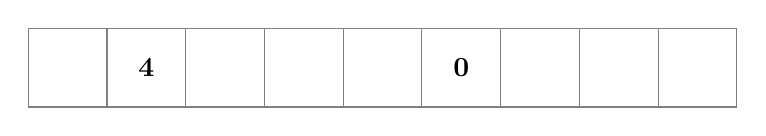
\begin{tikzpicture}
    \draw[step=1cm,color=gray] (0,0) grid (9,1);
    \node at (1.5,0.5) {\textbf{4}};
    \node at (5.5,0.5) {\textbf{0}};
\end{tikzpicture}
\end{figure}

We now perform the acceleration step for each vehicle. The second cell vehicle is
currently at speed 4 - as the vehicle in front is only 3 cells away, it does not
accelerate. The sixth cell vehicle increments its speed from 0 to 1.

During the slow step, the second cell vehicle must reduce its speed from 4 to 3
so it does not hit the sixth cell vehicle.

\begin{figure}[!h]
\centering
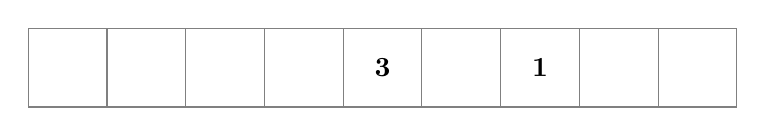
\begin{tikzpicture}
    \draw[step=1cm,color=gray] (0,0) grid (9,1);
    \node at (4.5,0.5) {\textbf{3}};
    \node at (6.5,0.5) {\textbf{1}};
\end{tikzpicture}
\end{figure}

Finally, the vehicles move to their new destinations. This demonstration breifly
shows the behaviour of two vehicles, but fails to demonstrate the creation and
flow of traffic jams. In Figure \ref{nagel-demo}, we can see how traffic jams
form and move in the Nagel-Schreckenberg model. This graph shows what happens
when there is a density of 0.1 cars per cell.

\begin{figure}[h]
    \centering
    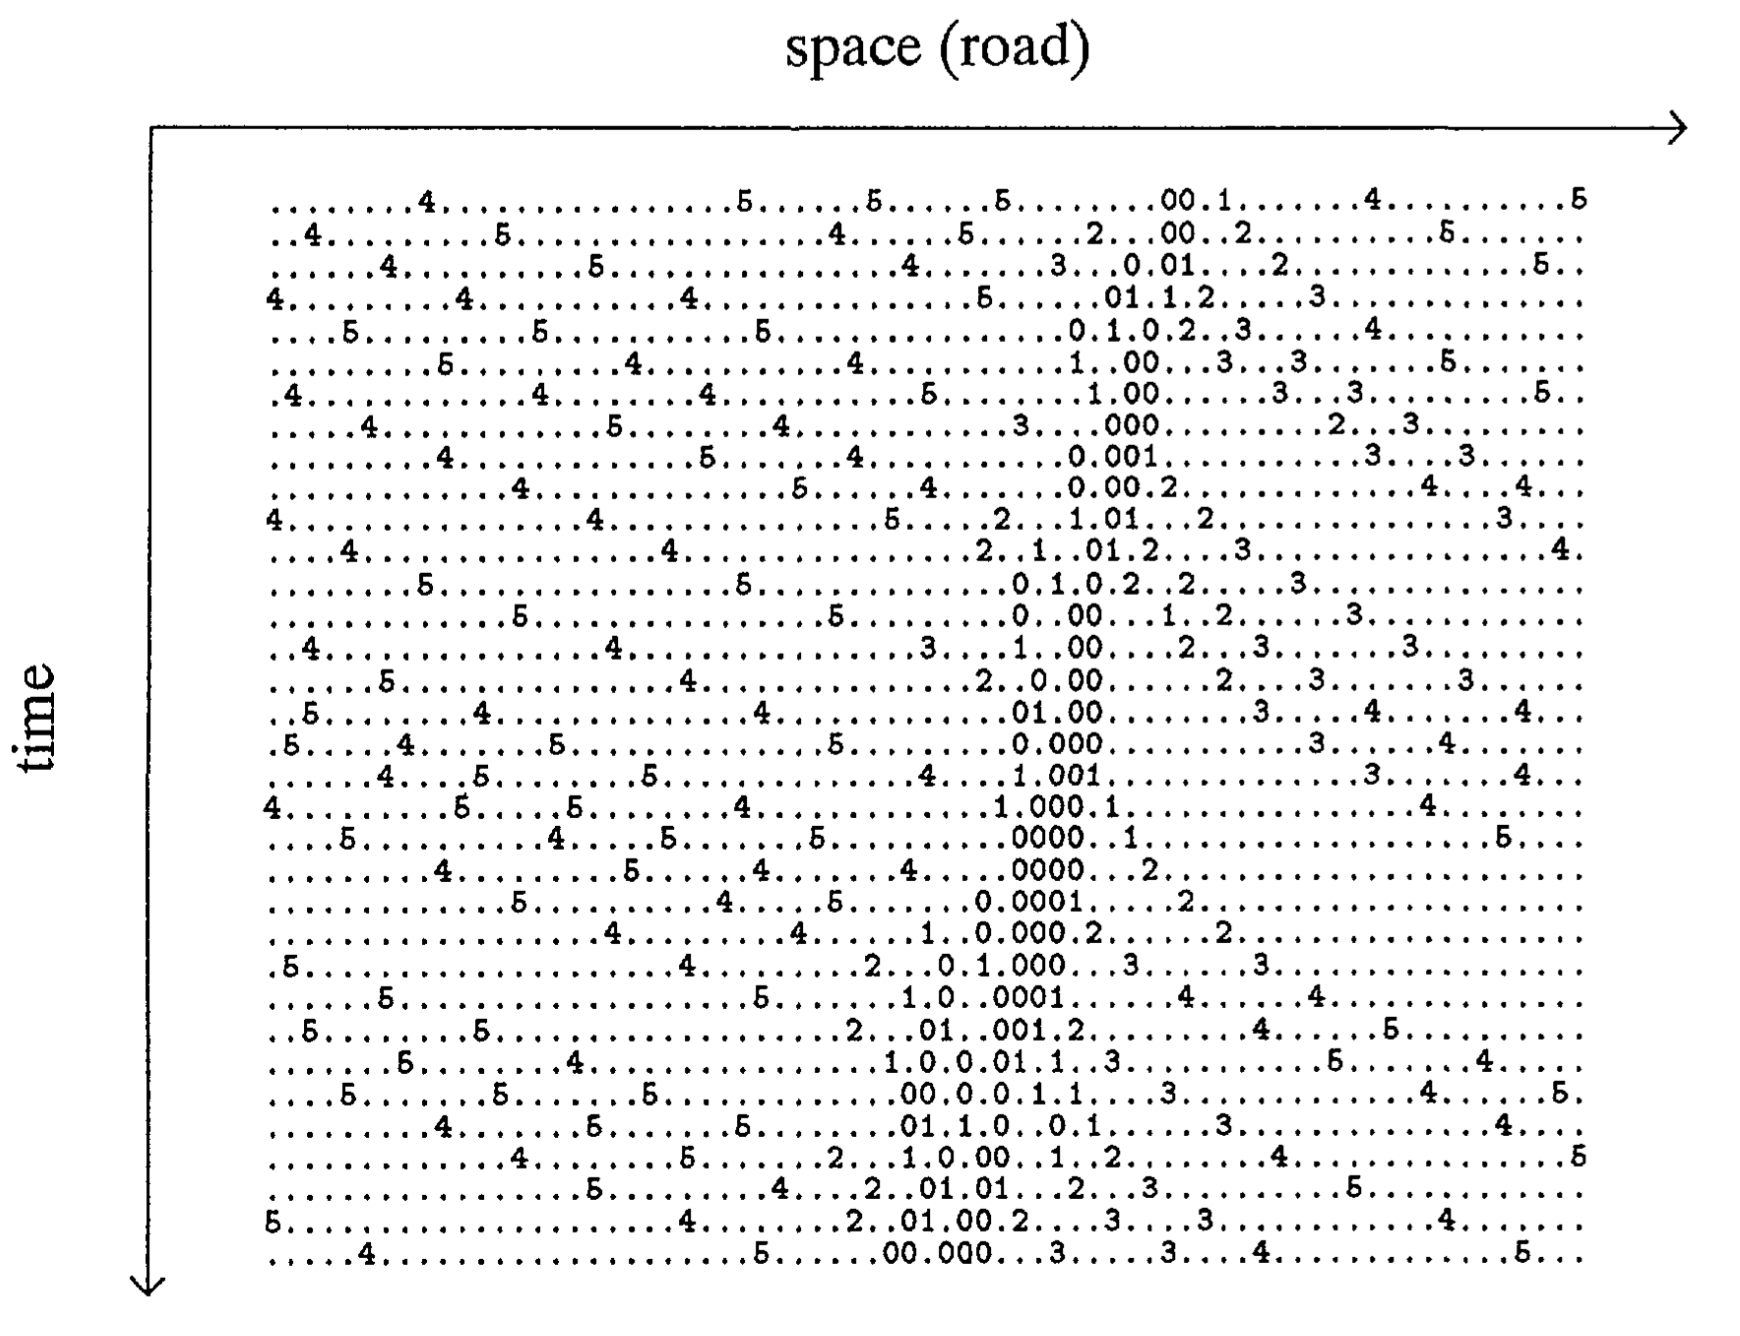
\includegraphics[scale=0.4]{nagel}
    \caption{Formation of traffic jams in the Nagel-Schreckenberg Model}\label{nagel-demo}
\end{figure}

%\textbf{Add info about n-lanes model if I decide to use that???}

\section{Implementation Background}

\subsection{OpenStreetMaps}

In OpenStreetMaps, there are three main elements - nodes, ways, and
relations. Each of these can have certain tags that describe the real-world
object they represent. For example, a way could have tags describing it as a
highway with 3 lanes, whilst a node could have tags identifying it as a
park bench or phone booth.

A standalone node is usually a single entity with a latitude and longitude as
well as an ID. By themselves, they can be used to represent small features such
as traffic lights, lampposts, or pylons. However, a way is also defined
by an ordered list of nodes.

Ways are the most flexible element in OpenStreetMaps. If a way starts and ends
at two different nodes, it is called an `open' way. This is commonly used for
sections of roads and paths. A way that starts and ends at the same node is
called a `closed' way. Often this is used to represent an area - such as a park
or the shape of a building - but can also be used for roundabouts and circular
barriers. There are tags for identifying if a closed way is an area or not
(primarly the \texttt{area=yes} tag, but many things are defined as areas even
without this tag).

Finally we have relations. These are the most complex type of element, holding
an ordered list of ways, nodes and other relations and have tags for describing
the relationship between them - for example, a bus route could be described as a
list of ways and nodes. For the purposes of routing, it is only important to
know that relations are used for turn restrictions - the rules that define which
directions a vehicle may move from one road onto another. This is important for
routing much more than mapping, as users would be frustrated to find that a
route they had expected to travel on is illegal or unsafe in practice.

\subsection{GraphHopper Routing Engine}

GraphHopper has been built to be fast, flexible and powerful. It covers the full
flow of creating a custom routing service - from parsing and importing
OpenStreetMaps data, processing the network for performance improvements,
routing using multiple dijkstra and A* algorithms and running a web server for
making requests. Additionally, it has built in support for car,
bicycle, pedestrian and other types of travel as well as the ability to create
custom vehicle types.

\begin{figure}[p]
    \centering
    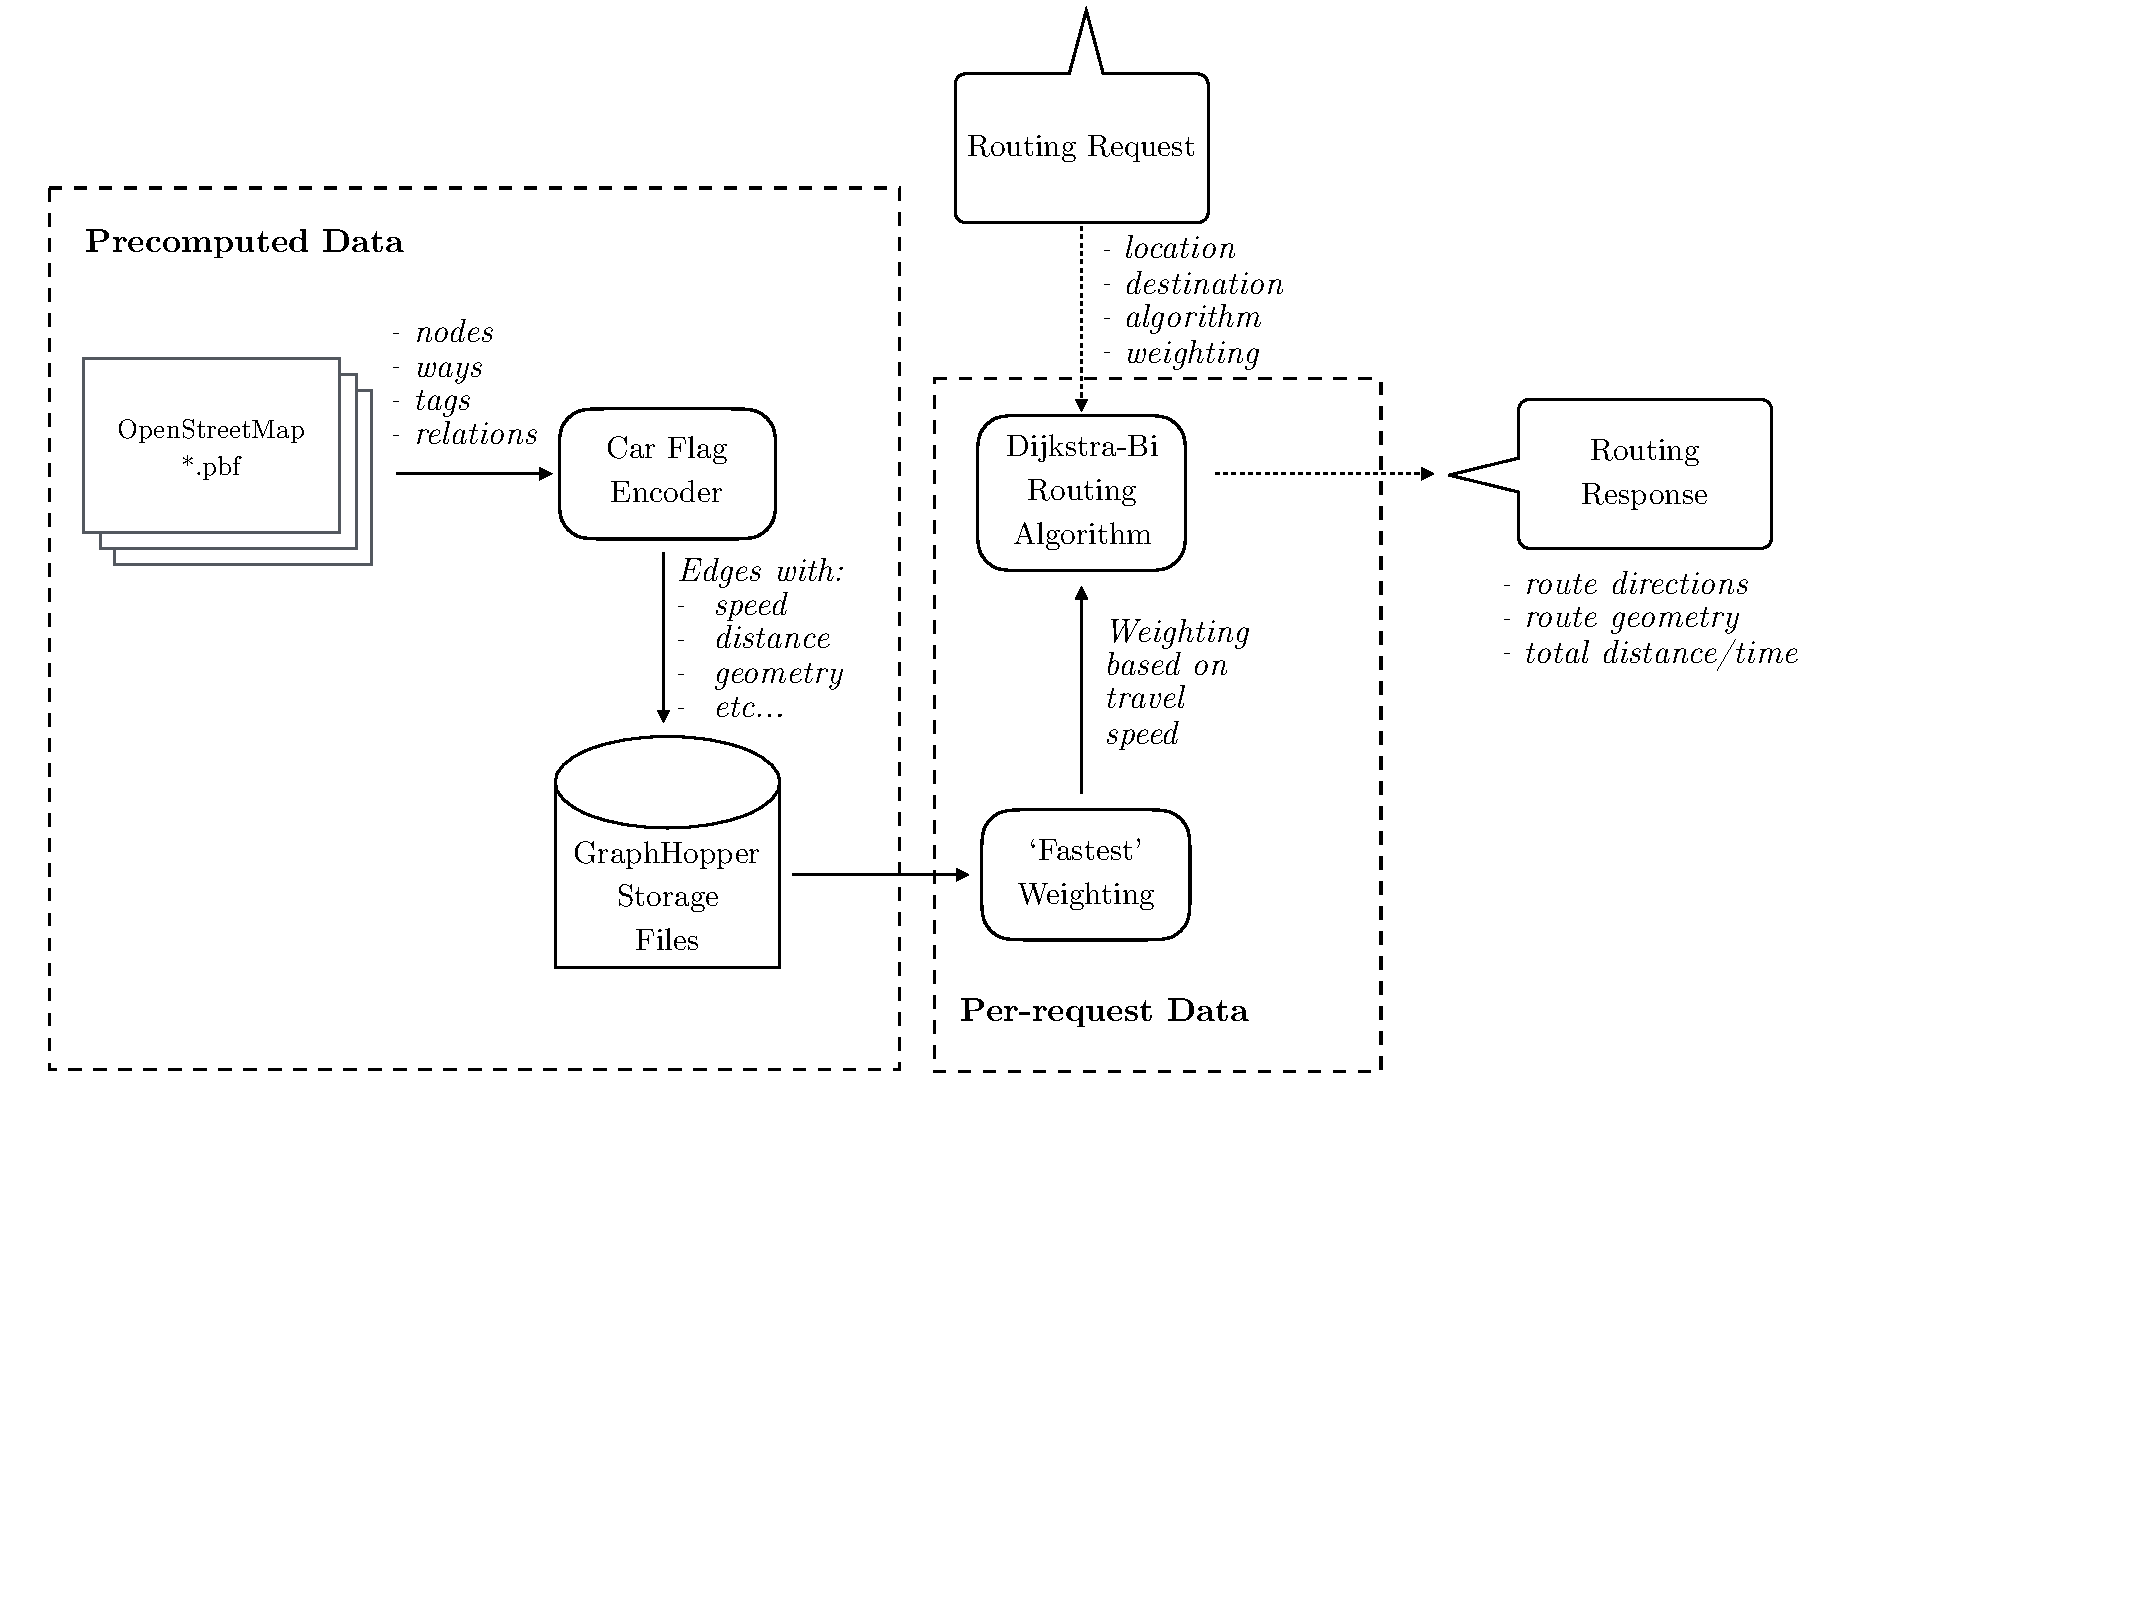
\includegraphics[scale=0.5,page=1,clip,trim=0 8cm 4cm 0]{architecture}
    \caption{An overview of the GraphHopper Architecture}\label{fig:gh-arch}
\end{figure}

Figure \ref{fig:gh-arch} shows the salient parts of the architecture for this project.
Note that we are not using the web or android modules, so no
details regarding their functionality has been included. For the most part, the
use of routing will be relatively high level - simply requesting a list of edges
between two points. However, the underlying engine also has a number of
features that make it easy to customise, which will be used for more complex
situations.

It is important to note that the conversion from OSM data to GraphHopper data
is done only once (as it is a time consuming process) and stores its results
on disk.

\subsubsection{OpenStreetMap Encoding}

\begin{figure}[p]
    \centering
    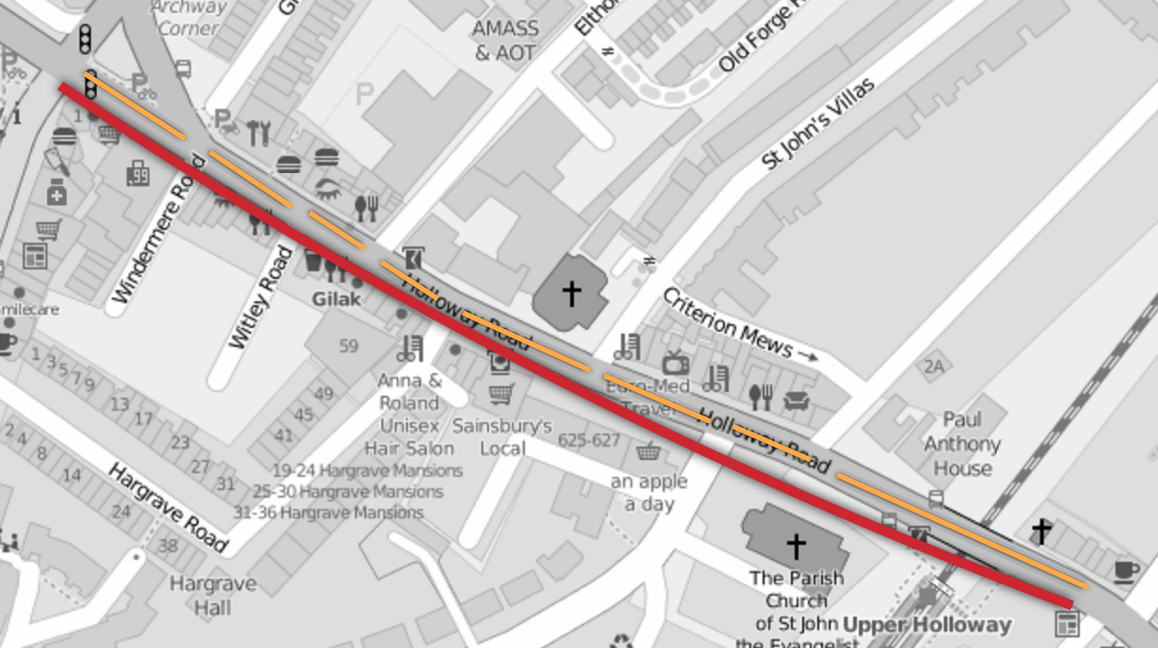
\includegraphics[scale=0.6]{osm-gh}
    \caption{OpenStreetMap way representation compared to edges in GraphHopper}\label{fig:osm-gh}
\end{figure}

The first thing to understand is how GraphHopper converts the OpenStreetMap data
into a graph that can be used for routing.
For the purposes of routing, we are primarily concerned with ways that represent
roads. However, a way does not represent the entirety of a given road - but is
also not granular enough to allow routing. Figure \ref{fig:osm-gh} shows the
difference between ways, roads and edges. We can see that Holloway Road extends
beyond the OSM way in red. However, if we used the way for routing we could not
route from Hargrave Road to St John's Villas via Holloway Road. To perform
routing, GraphHopper splits every way into multiple edges whenever there is a
junction of any kind - these can be seen in orange. We can now perform the
routing calculation mentioned before - there is now an edge along a subsection of
Holloway Road that conncets Hargrave Road to St John's Villas.

\subsubsection{Flag Encoders}

Internally, GraphHopper compresses the information about each edge into a
single integer - so each edge takes up no more than 32 or 64 bits.

The \texttt{FlagEncoder} interface (and the \texttt{AbstractFlagEncoder} class) define what
operations have to be done to convert a section of a way into an edge. Edges
store a few key pieces of information - by default, GraphHopper stores the
length, speed and ID of an edge, with additional information optionally stored
by the flag encoder itself.

For example, the \texttt{CarFlagEncoder} uses the type of road to calculate the
correct maximum speed of the vehicle and then sets the speed for the edge, using
5 bits. The \texttt{MotorcycleFlagEncoder} can do the same thing, but with
different speed values for each type of road. The concept can be extended to
storing even more information at each edge - for example, 3D graph data can be
stored for bike and walking routes, whilst a FlagEncoder for trucks could store
height, weight, width and length restrictions to ensure safe travel.

\subsubsection{Weightings}

Flag Encoders are used to define what information can be used whilst routing -
but this data is fixed once the OSM file has been processed. A weighting defines
how the data stored at the edges is used. For example, one can search for the
shortest route, the fastest route, or a custom weighting that incorporates other
information stored in the edge.

% -----------------------------------------------------------------------------

\chapter{Project Execution}
\label{chap:execution}

%%%%%% ======= 15 PAGES ======= %%%%%%

\definecolor{mygreen}{rgb}{0,0.6,0}
\definecolor{mygray}{rgb}{0.5,0.5,0.5}
\definecolor{mymauve}{rgb}{0.58,0,0.82}

\lstset{ %
  backgroundcolor=\color{white},   % choose the background color
  basicstyle=\footnotesize\ttfamily,        % size of fonts used for the code
  breaklines=true,                 % automatic line breaking only at whitespace
  captionpos=b,                    % sets the caption-position to bottom
  commentstyle=\color{mygreen},    % comment style
  escapeinside={\%*}{*)},          % if you want to add LaTeX within your code
  keywordstyle=\color{blue},       % keyword style
  stringstyle=\color{mymauve},     % string literal style
  language=Java
}


\section{Project Setup and Modularisation}

When setting up the project, it was important to be able to use and modify the
underlying GraphHopper routing engine. The GraphHopper project is setup with
four existing modules - core, tools, web and android. Although it would have
been ideal to use GraphHopper as an external library, it was necessary to make
minor internal changes to the main engine. As such, I created a GitHub fork of
the project and added a new module for the project, called marmoset.

This allowed me to use GraphHopper as a library for the majority of tasks, but
was still able to modify the visibility of certain methods that were necessary
for the tasks I wanted to perform.

GraphHopper uses the Maven dependency and build tool, with its own custom shell
script for building, running and testing different versions of the engine. To
keep separation from the core project, I created my own shell script for
building and running the marmoset engine. It supports four main actions - clean,
build, rebuild and run. It also allows multiple commands to be run in succession
for convenience.

Additionally, I wanted to create a modern codebase in spite of the core engine
being written in Java. Although I briefly explored using Scala, much of my work
would rely on extending and using the existing Java APIs in GraphHopper.
Thankfully, Java 8 has introduced a number of key tools that allow
functional-style code to be written. The code below shows the difference for
performing a simple task - converting a list of objects into strings and joining
them by commas.

\noindent
\begin{tabular}{c|c}

\begin{lstlisting}
public String getVehicleData()
{
    StringBuilder sb = new StringBuilder();
    for (VehicleController v : vehicles)
    {
        sb.append(v.getVehicle().toString());
        sb.append(",");
    }
    // remove last comma
    sb.deleteCharAt(sb.length() - 1);
    return sb.toString();
}
\end{lstlisting} &
\begin{lstlisting}[boxpos=b]
public String getVehicleString()
{
    return vehicles.stream()
        .map(Vehicle::toString)
        .collect(Collectors.joining(","));
}
\end{lstlisting} \\ \vspace{1em}
Java 7 Implementation & Java 8 Implementation \\
\end{tabular}

Here we can see how six lines of code can be condensed into a single, more
readable line using the Java 8 Stream API.

\section{Initial Client-Server setup}

There are two key parts of the simulation engine - a front end visualisation and
a back end simulation. The first thing to do was create a server and find an
efficient way of sending simulation data to the front end.

For the raw file server, I used the NanoHttd~\cite{nanohttpd} library, as it
required minimal setup and is easy to run on a separate thread. For the
client-server communication, I initially used the NanoHttpd WebSocket
implementation, but it did not appear to be fully functional. As such, I
switched to using the Java-Websocket library~\cite{javawebsocket}, extending the
WebSocketServer class to implement my own protocol on top of WebSocket.

\subsection{Initial API design}

\subsection{Routing Behaviour}

\subsection{Multi-Vehicle Support}

\section{Cell Automata Model}

Test

\subsection{Vehicle and Cell Iterators}

Test

\section{Performance Improvements}

Test

\subsection{Binary vs String data}

Test

\subsection{Removing animations}

Test

\subsection{Removing timelock}

Test

\subsection{DOM to Canvas}

Test

\subsection{Parallel processing}

Test

\subsection{Metric calculations}

%This chapter is intended to describe what you did: the goal is to explain
%the main activity or activities, of any type, which constituted your work
%during the project.  The content is highly topic-specific, but for many
%projects it will make sense to split the chapter into two sections: one
%will discuss the design of something (e.g., some hardware or software, or
%an algorithm, or experiment), including any rationale or decisions made,
%and the other will discuss how this design was realised via some form of
%implementation.

%This is, of course, far from ideal for {\em many} project topics.  Some
%situations which clearly require a different approach include:

%\begin{itemize}
%\item In a project where asymptotic analysis of some algorithm is the goal,
      %there is no real ``design and implementation'' in a traditional sense
      %even though the activity of analysis is clearly within the remit of
      %this chapter.
%\item In a project where analysis of some results is as major, or a more
      %major goal than the implementation that produced them, it might be
      %sensible to merge this chapter with the next one: the main activity
      %is such that discussion of the results cannot be viewed separately.
%\end{itemize}

%\noindent
%Note that it is common to include evidence of ``best practice'' project
%management (e.g., use of version control, choice of programming language
%and so on).  Rather than simply a rote list, make sure any such content
%is useful and/or informative in some way: for example, if there was a
%decision to be made then explain the trade-offs and implications
%involved.

% -----------------------------------------------------------------------------

\chapter{Critical Evaluation}
\label{chap:evaluation}

%{\bf A topic-specific chapter, of roughly $15$ pages}
%\vspace{1cm}

%\noindent
%This chapter is intended to evaluate what you did.  The content is highly
%topic-specific, but for many projects will have flavours of the following:

%\begin{enumerate}
%\item functional  testing, including analysis and explanation of failure
      %cases,
%\item behavioural testing, often including analysis of any results that
      %draw some form of conclusion wrt. the aims and objectives,
      %and
%\item evaluation of options and decisions within the project, and/or a
      %comparison with alternatives.
%\end{enumerate}

%\noindent
%This chapter often acts to differentiate project quality: even if the work
%completed is of a high technical quality, critical yet objective evaluation
%and comparison of the outcomes is crucial.  In essence, the reader wants to
%learn something, so the worst examples amount to simple statements of fact
%(e.g., ``graph X shows the result is Y''); the best examples are analytical
%and exploratory (e.g., ``graph X shows the result is Y, which means Z; this
%contradicts [1], which may be because I use a different assumption'').  As
%such, both positive {\em and} negative outcomes are valid {\em if} presented
%in a suitable manner.

% -----------------------------------------------------------------------------

\chapter{Conclusion}
\label{chap:conclusion}

%{\bf A compulsory chapter,     of roughly $5$ pages}
%\vspace{1cm}

%\noindent
%The concluding chapter of a dissertation is often underutilised because it
%is too often left too close to the deadline: it is important to allocation
%enough attention.  Ideally, the chapter will consist of three parts:

%\begin{enumerate}
%\item (Re)summarise the main contributions and achievements, in essence
      %summing up the content.
%\item Clearly state the current project status (e.g., ``X is working, Y
      %is not'') and evaluate what has been achieved with respect to the
      %initial aims and objectives (e.g., ``I completed aim X outlined
      %previously, the evidence for this is within Chapter Y'').  There
      %is no problem including aims which were not completed, but it is
      %important to evaluate and/or justify why this is the case.
%\item Outline any open problems or future plans.  Rather than treat this
      %only as an exercise in what you {\em could} have done given more
      %time, try to focus on any unexplored options or interesting outcomes
      %(e.g., ``my experiment for X gave counter-intuitive results, this
      %could be because Y and would form an interesting area for further
      %study'' or ``users found feature Z of my software difficult to use,
      %which is obvious in hindsight but not during at design stage; to
      %resolve this, I could clearly apply the technique of Smith [7]'').
%\end{enumerate}

% =============================================================================

% Finally, after the main matter, the back matter is specified.  This is
% typically populated with just the bibliography.  LaTeX deals with these
% in one of two ways, namely
%
% - inline, which roughly means the author specifies entries using the
%   \bibitem macro and typesets them manually, or
% - using BiBTeX, which means entries are contained in a separate file
%   (which is essentially a databased) then inported; this is the
%   approach used below, with the databased being dissertation.bib.
%
% Either way, the each entry has a key (or identifier) which can be used
% in the main matter to cite it, e.g., \cite{X}, \cite[Chapter 2}{Y}.

\backmatter

\bibliography{dissertation}

% -----------------------------------------------------------------------------

% The dissertation concludes with a set of (optional) appendicies; these are
% the same as chapters in a sense, but once signaled as being appendicies via
% the associated macro, LaTeX manages them appropriatly.

\appendix

\chapter{An Example Appendix}
\label{appx:example}

%Content which is not central to, but may enhance the dissertation can be
%included in one or more appendices; examples include, but are not limited
%to

%\begin{itemize}
%\item lengthy mathematical proofs, numerical or graphical results which
      %are summarised in the main body,
%\item sample or example calculations,
      %and
%\item results of user studies or questionnaires.
%\end{itemize}

%\noindent
%Note that in line with most research conferences, the marking panel is not
%obliged to read such appendices.

% =============================================================================

\end{document}
